%!TEX root = ../report.tex

% 
% Architecture
% 

% 2/3 pages
%Your proposed architecture. Can have lots of pictures and 
% bullet points so it is easy to understand.
\section{Architecture}
\label{sec:architecture}
We propose a framework, to develop mobile web apps for smart
places, that allow developers to only write the code
for the application logic and the specific behavior when
the user is nearby specific points of interest (POI).
Each beacon represents one POI. Developers would not need
to write the code that gets beacons' data and get the
right information from a back-end. They would need only
to write the code for each specific POI. They could give
a name to each POI and the app will receive that name 
instead of the beacon's raw data. 

Since mobile web apps do not need to be installed, 
we choose to support
them instead of native, to allow
the user to have access to any app in any smart place.
This apps run on the device's browser. However, detecting
nearby beacons is not a feature integrated in the mobile
Operating System. Our solution would be to build the
Smart Places App,
that detects nearby beacons, turn them into names and
other high-level information, and deliver it to the
mobile web app. The user would need only this app to
be able to access any smart place app. Also, the same app
could be used to configure a smart place.
For instance, a restaurant's owner wants to offer, to
his customers, the possibility to make their orders,
as soon as they sit, from their smartphones. Some
developers, could develop the app for restaurants,
using our framework. These developers would only think
about tables instead of beacons. The owner would need
to put a beacon in each table. After the beacons
installation, he could just use the Smart Places App,
choose the app for restaurants, and put his smartphone
closer to a beacon and configure it. This configuration
would be, for each beacon, what is the number of the table
where it is deployed. Then, his customers would only
need the Smart Places App, turn on bluetooth and they will
be notified that they can make their orders from their
smartphones.

%Solution overview
Our solution has three main components,
the BLE Beacons, as it is shown in figure 
\ref{fig:overview_architecture}, 
the Back-end and an Android app
that will run on the users' smartphones.
\begin{figure}[!ht]
  \centering
    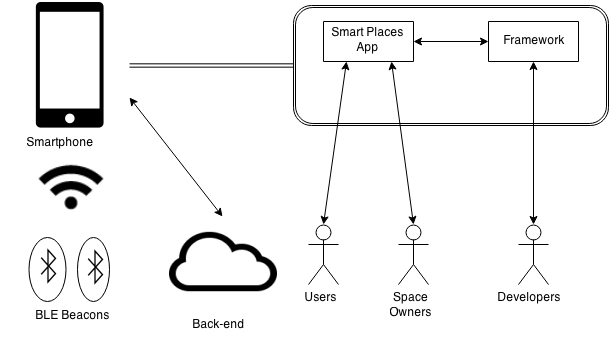
\includegraphics[width=0.9\textwidth]{img/overview_architecture}
    \caption{Overview of the solution}
    \label{fig:overview_architecture}
\end{figure}
The \textbf{BLE Beacons}, as it is explained in section 
\ref{sec:introduction}, are small devices that broadcast
an ID using Bluetooth Low Energy. The \textbf{Backend} is where information about each beacon is stored. 
And, the users'
\textbf{smartphones}, where the \textbf{Smart Places App} will run.
It is a native Android app that will scan for nearby beacons,
get the information about them from the Back-end and
provide that information to the app associated to a 
given Smart Place.
\textbf{Users} will use this app to have access
to any app running in any Smart Place.
Also, \textbf{Smart Places Owners} can use it to configure
their Smart Places and configure which applications
will run there.
Since these apps will be mobile web apps, they will run
in a embedded browser inside the Smart Places App.
\textbf{Developers} will need to use the \textbf{Framework} to
develop such apps. Also, the Framework will provide an
Interface between the mobile web app, that will run
in a given Smart Place, and the Smart Places App.
Figure \ref{fig:architecture} shows the two main
blocks that will run inside the smartphone.
We have the Smart Places App and the Framework itself.
\begin{figure}[!ht]
  \centering
    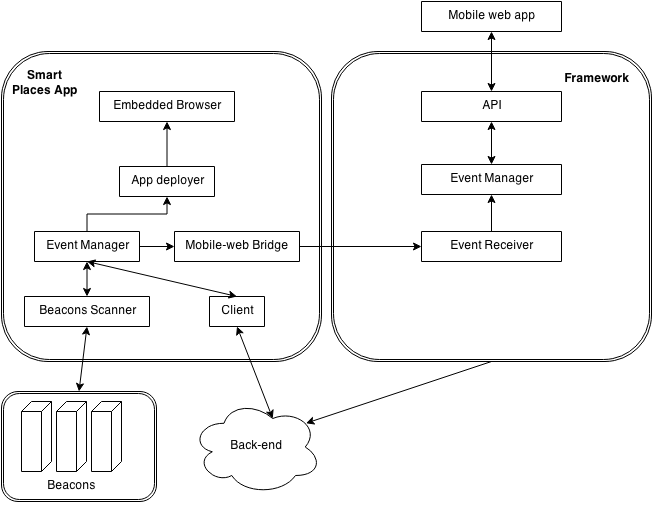
\includegraphics[width=0.9\textwidth]{img/architecture}
    \caption{Architecture}
    \label{fig:architecture}
\end{figure}

\subsection{Smart Places App}
\label{sub:smart_places_app}
As already mentioned, the Smart Places App will be a native
Android app that the user and the Smart Place Owner will use,
in order to be able to use any app of any Smart Place
and configure a Smart Place, respectively.
The \textbf{Beacons Scanner} will scan for nearby
beacons. After scanning, it will deliver the IDs
of the beacons to the \textbf{Beacons Manager}.
The Beacons Manager will call the \textbf{Client} to
get the information about each POI that is being
represented by each beacon from the back-end or
from the \textbf{Beacons Cache}. It will be possible to
configure the Smart Places App to use the cache or not.
This cache will be an optimization to avoid communication
with the back-end in each scan. If this cache is being
used, when a scan is completed, the Client will
check if the information about that beacon is in
the cache. If it is, the Client do not need to request
from the back-end. Otherwise, the Client will
request the information about all the POIs of that
Smart Place. In the next beacons scan, if we stay in
the same Smart Place, there is no need make requests
to the back-end since all the mapping between beacons
and POIs is in the cache.
If no cache is used, the Client will always make requests
to the back-end in each beacon scan.
After getting the POI information from the Client,
the Beacons Manager will call the \textbf{Mobile-web bridge},
which provides an interface between the native app
and the web app, that will deliver this information
to the mobile web app that is running in the
\textbf{Embedded Browser}. 
Each time the web app needs to interact
with the native app, this component is called.
The \textbf{User Manager} is called to login the
user and to get the information about the logged
in user. To perform the user's login, the User Manager
will call the Client that will send the needed information
to the back-end to login the user. After this step,
the mobile web app, can use the Mobile-web bridge
to get information about the logged in user.

\subsection{Framework}
\label{sub:framework}
The Framework provides, to developers, an \textbf{API} that they
can use to perform operations about the POIs or about the users.
The API uses the \textbf{User Manager} when developers want to
get information about the logged in user.
Developers are allowed to define callbacks for each POI or to
even create new POIs. In order to do this, the API
uses the \textbf{POIs Manager} that will store the callbacks
for each POI.
